En este capítulo se resume el proceso de desarrollo del sistema elaborado, detallando los principales componentes que lo conforman y su funcionamiento. 
La explicación se estructura siguiendo el orden real de la implementación del proyecto, comenzando por el desarrollo del frontend, seguido de la creación de la base de datos y la construcción del backend. 
Finalmente, se comentan los distintos servicios integrados en la aplicación, como el envío de correos electrónicos, el bot de Discord, la conexión con la IA mediante Dialogflow y la automatización de los trámites con funciones de RPA. 

\section{Implementación del frontend}
    Para el desarrollo del frontend de la aplicación se ha utilizado el sistema de plantillas de Jinja. 
    Se ha definido una plantilla base (layout.jinja), mostrada en la figura \ref{fig:5.1}, que funciona como estructura común para todas las vistas de la web. 
    \begin{figure}[H]
        \centering
        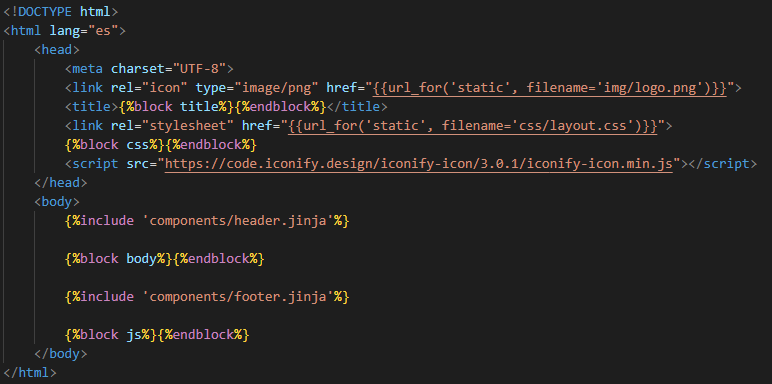
\includegraphics[width=0.75\textwidth]{img/desarrollo/layout.png}
        \caption{Código de la plantilla base layout.jinja.}
        \label{fig:5.1}
    \end{figure}
    Esta plantilla incluye componentes reutilizables del sistema, como la cabecera y el pie de página, permitiendo que el resto de vistas definan únicamente el contenido específico. 
    Este enfoque reduce la duplicación de código y mejora la mantenibilidad del sistema, facilitando las modificaciones globales.

    Asimismo, se importa una hoja de estilos CSS común para toda la aplicación, garantizando coherencia visual en todas las páginas mediante el uso de la misma paleta de colores, tipografía y estructura. 
    
    Por último, se integra la librería de iconos open source \href{https://iconify.design/}{Iconify} \cite{ref15}, lo que permite incorporar iconos de forma sencilla en las distintas vistas.

    Cabe destacar que el frontend incluye múltiples vistas con sus hojas de estilos y scripts dinámicos. 
    Sin embargo, en esta sección se comentan únicamente los elementos más representativos técnicamente, evitando detallar componentes HTML simples o repetitivos, o estilos o validaciones sin importancia. 

    \begin{figure}[H]
        \centering
        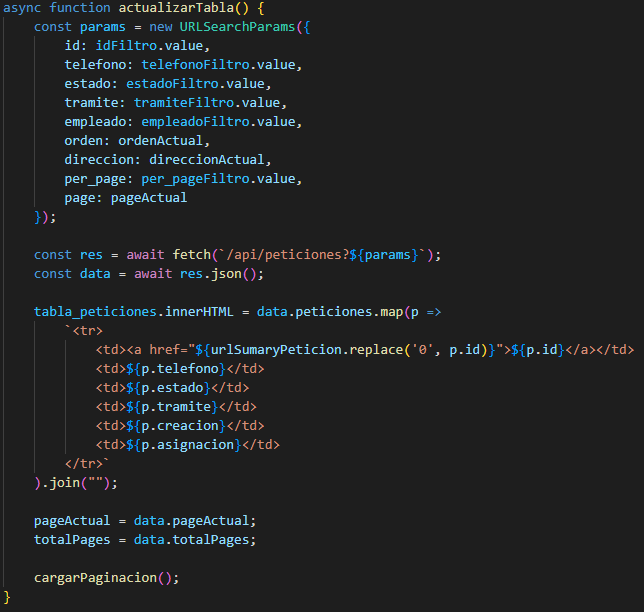
\includegraphics[width=0.75\textwidth]{img/desarrollo/peticionesjs.png}
        \caption{Fragmento de código de la construcción dinámica de la tabla de peticiones.}
        \label{fig:5.2}
    \end{figure}
    Los componentes principales de la web son las tablas que muestran la información correspondiente a las peticiones, empleados o trámites. 
    El contenido de estas tablas se carga dinámicamente en función de los los filtros, el orden o la paginación. 
    La figura \ref{fig:5.2} muestra el fragmento de código en el que se llama a un endpoint, "/api/peticiones", para recuperar la información correspondiente de la base de datos y actualizarla en la tabla.

    \begin{figure}[H]
        \centering
        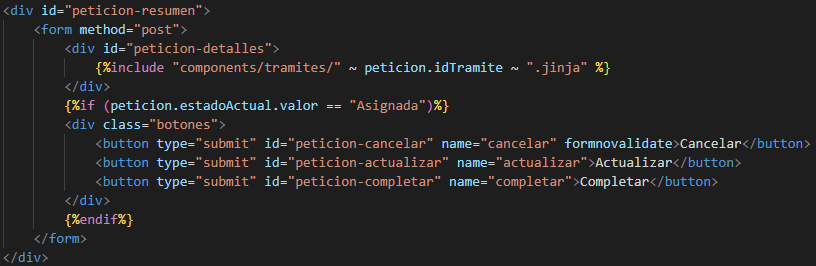
\includegraphics[width=0.75\textwidth]{img/desarrollo/sumaryPeticion.png}
        \caption{Fragmento de código de la plantilla resumen de una petición.}
        \label{fig:5.3}
    \end{figure}
    \begin{figure}[H]
        \centering
        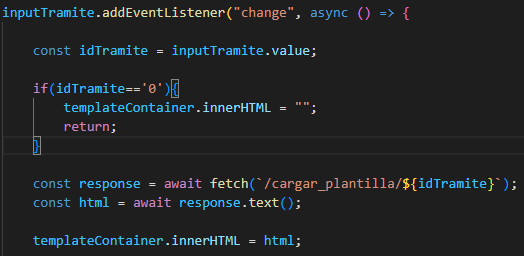
\includegraphics[width=0.6\textwidth]{img/desarrollo/crearPeticionjs.png}
        \caption{Fragmento de código de carga dinámica de las plantillas de cada trámite.}
        \label{fig:5.4}
    \end{figure}
    De forma análoga, las plantillas que contienen la información correspondiente a cada trámite se renderizan en tiempo de ejecución, mostrando el formulario correspondiente dependiendo del trámite escogido, figuras \ref{fig:5.3} y \ref{fig:5.4}. 

    El resto de componentes que abundan en la aplicación son formularios, que no presentan nada especial salvo alguna validación o evento dinámico.

\section{Implementación de la base de datos}
    La implementación de la base de datos se ha llevado a cabo mediante tablas SQL, definiendo en cada atributo su tipo de dato, restricciones de unicidad y posibilidad de valores nulos. 
    Asimismo, se han establecido las claves primarias para cada tabla y las claves foráneas para modelar las relaciones entre entidades.

    La figura \ref{fig:5.5} muestra la función encargada de inicializar la base de datos en la aplicación, ejecutando el archivo SQL correspondiente durante el arranque del sistema. 
    \begin{figure}[H]
        \centering
        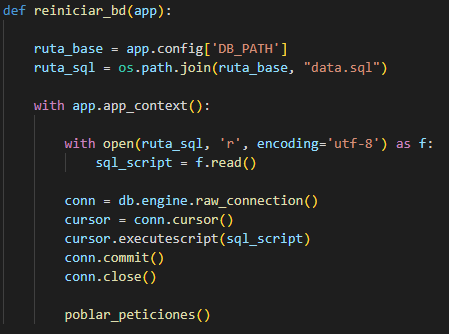
\includegraphics[width=0.6\textwidth]{img/desarrollo/utils_db.png}
        \caption{Código de la función de inicialización de la base de datos.}
        \label{fig:5.5}
    \end{figure}

    Para gestionar la base de datos dentro de la aplicación se utiliza SQLAlchemy, lo que permite definir clases Python equivalentes a cada tabla y trabajar con los registros como objetos. 
    La figura \ref{fig:5.6} muestra un ejemplo de consulta dinámica sobre la tabla de peticiones, en la que se aplican filtros, ordenación y paginación en función de los parámetros recibidos. 
    El resultado se almacena en la variable "peticiones" como una lista de objetos de la clase correspondiente, permitiendo acceder a sus atributos y métodos directamente.
    \begin{figure}[H]
        \centering
        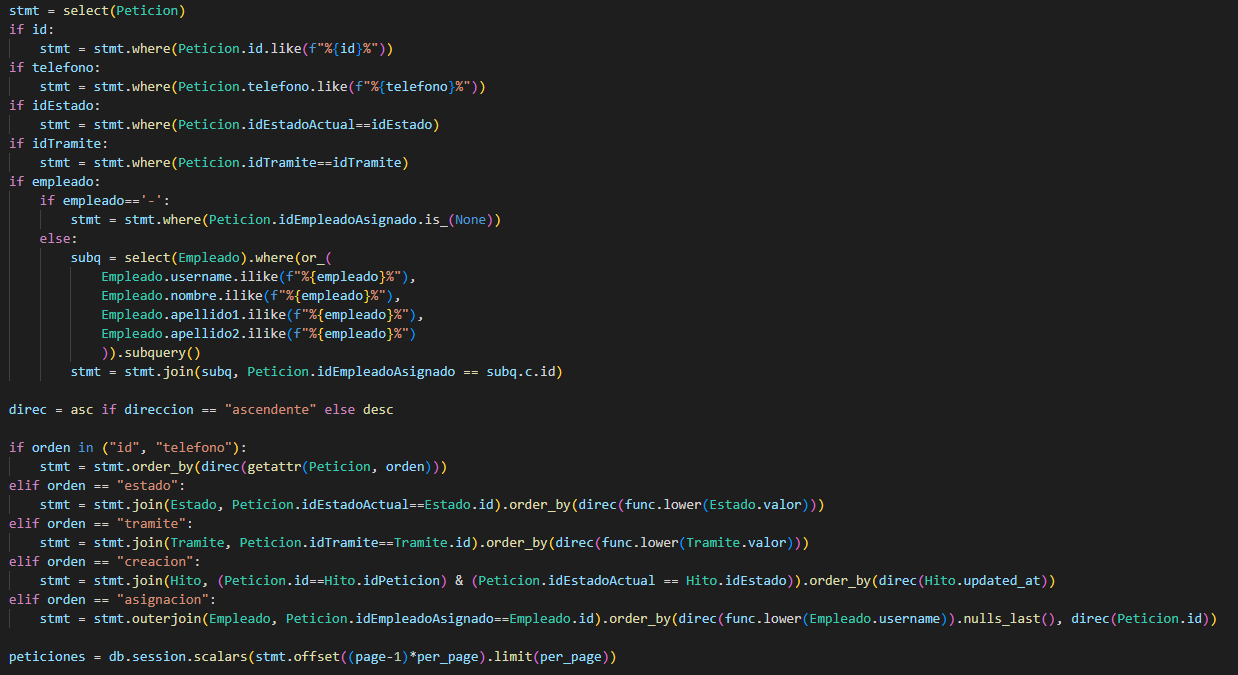
\includegraphics[width=1\textwidth]{img/desarrollo/dashboard.png}
        \caption{Fragmento de código de la consulta de peticiones.}
        \label{fig:5.6}
    \end{figure}

\section{Implementación del backend}
    En esta sección se va a tratar el desarrollo del backend de la aplicación web, centrándolo en las rutas que ejercen como controladores de las vistas. 
    Por modularidad, se han definido distintos blueprints para cada parte de la aplicación, permitiendo organizar el código de forma más clara dividiendo las rutas y su lógica en distintos archivos Python. 
    
    El primer blueprint es el de inicio, que se encarga de redireccionar al inicio de sesión. 
    También incluye un endpoint que renderiza la plantilla con la información de cada trámite, llamado dinámicamente desde el formulario de crear peticiones. 

    El segundo blueprint es el de autenticación, que incluye las rutas para iniciar y cerrar sesión. 
    Las sesiones se gestionan mediante la extensión Flask-Login, que incluye funciones que simplifican la gestión de usuarios identidficados, como el decorador @login\_required, que se escribe en las funciones de las rutas para bloquear el acceso a usuarios no autenticados. 
    Además, se ha implementado un sistema de permisos para cada rol, figura \ref{fig:5.7}, que se almacenan en un archivo JSON y se cargan en la sesión de cada usuario cuando se identifican. 
    La figura \ref{fig:5.8} muestra el código de las funciones que gestionan los permisos, incluido un decorador personalizado, @permiso\_requerido, que actua de forma análoga a @login\_required, bloqueando el acceso a las rutas a las que el usuario no tenga permiso.
    \begin{figure}[H]
        \centering
        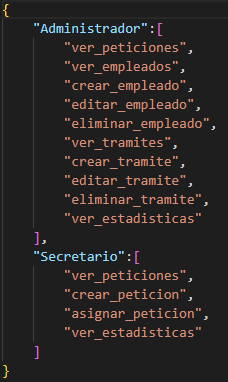
\includegraphics[width=0.2\textwidth]{img/desarrollo/permisosjson.png}
        \caption{JSON con los permisos de cada rol.}
        \label{fig:5.7}
    \end{figure}
    \begin{figure}[H]
        \centering
        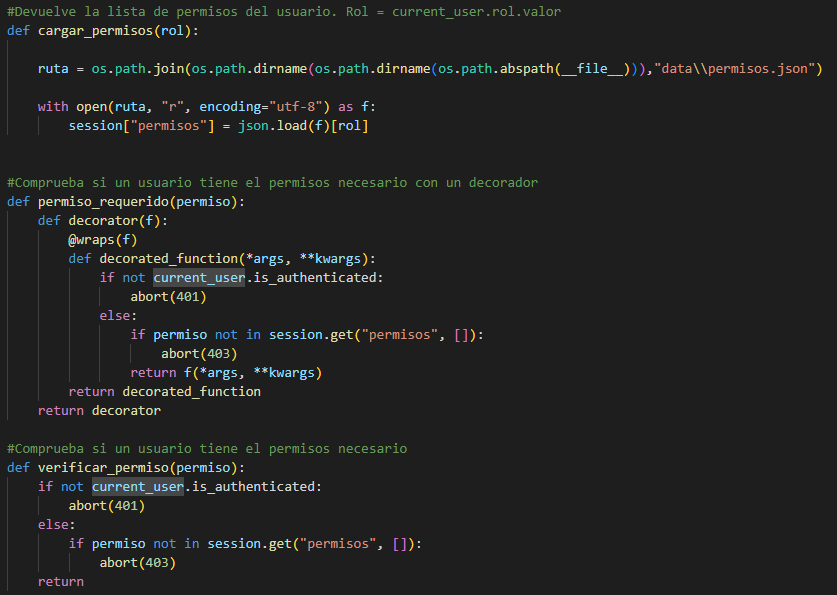
\includegraphics[width=0.7\textwidth]{img/desarrollo/permisospy.png}
        \caption{Código de las funciones para la gestión de permisos en la aplicación.}
        \label{fig:5.8}
    \end{figure}

    El tercer blueprint es el más importante, incluye las rutas que gestionan las vistas y funcionalidades principales de la aplicación. 
    En este módulo se encuentran las funciones que gestionan las peticiones, empleados, trámites y la información del perfil de cada empleado. 
    Estas funciones incluyen principalmente la lógica para recuperar la información necesaria de la base de datos, como en la figura \ref{fig:5.6}, renderizar las plantillas correspondientes y gestionar la información recibida de los formularios. 
    
    Tanto las peticiones como los empleados y trámites se gestionan de forma similar en el backend, ya que comparten la forma en la que se presentan en el frontend.
    En los tres casos se ha implementado una ruta para renderizar la página con la tabla y un endpoint para recuperar la información de la tabla en formato JSON. 
    En el supuesto de las peticiones se ha añadido una ruta para mostrar el resumen de cada petición, con la funcionalidad correspondiente para asignarse la petición, completarla, cancelarla, editarla o desasignársela, y otra ruta independiente para crear nuevas peticiones.
    Sin embargo, en el caso de los empleados y trámites se simplifica la lógica reutilizando la misma ruta y plantilla tanto para mostrar los datos individuales y editarlos como para crear nuevos registros, diferenciando ambos casos mediante la presencia o ausencia de un ID en la URL.

    El cuarto blueprint sirve para gestionar la carga y subida de archivos en la web. 
    Hasta el momento, esta funcionalidad se utiliza únicamente para recuperar la imagen de perfil de cada empleado que se muestra tanto en el perfil como en el historial de cada petición. 
    También permite modificar la imagen de perfil, almacenando la imagen nueva y borrando la antigua. 

    Por último, hay un blueprint de errores, que se encarga únicamente de renderizar una plantilla personalizada en caso de error 404, es decir, cuando el empleado intenta acceder a un recurso inexistente, y de error 403, cuando el empleado intenta acceder a un recurso para el que no tiene permiso.
    
    Adicionalmente, se ha implementado otro blueprint independiente para modularizar la lógica de las APIs 
    Por el momento, este incluye un único endpoint que actúa como webhook para procesar los eventos de Dialogflow, cuya integración se comentará con mayor detalle en la sección siguiente.

\section{Implementación e integración de servicios}
    Esta sección se centra en explicar la implementación de los cuatro servicios integrados en la aplicación, poniendo especial atención en aquellos relacionados con la gestión de las llamadas, ya que constituyen el eje central del proyecto. 
    
    \subsection{Implementación e integración del servicio de correo electrónico}
        Para la gestión del envío de correos electrónicos dentro de la aplicación web se ha utilizado la extensión Flask-Mail, que permite integrar facilmente un sistema de notificaciones por correo electrónico dentro del framework Flask. 
        Este servicio se utiliza para comunicar automáticamente a los empleado distinta información relacionada con su cuenta, como el envío de sus credenciales de acceso, el establecimiento de una nueva contraseña temporal o la activación y desactivación del acceso al sistema. 

        Teniendo en cuenta el alcance del proyecto, no se ha configurado un servidor de correo real. 
        En su lugar, se ha utilizado un servidor SMTP local de pruebas ejecutado en localhost mediante la herramienta aiosmtpd. 
        De esta forma, los correos generados por la aplicación se muestran por consola, lo que permite verificar su correcto funcionamiento sin necesidad de utilizar un servidor real. 

        Finalmente, la configuración actual del servicio de correo electrónico se encuentra en el archivo config.py, donde se definen los parámetro necesarios para su funcionamiento, siendo fácilmente modificable para la futura integración del servidor real que se utilice en producción. 
        El envío de correos se realiza de forma centralizada mediante una única función, figura \ref{fig:5.9}, lo que permite generar distintos tipos de mensajes ajustando únicamente los parámetros de entrada. 
        \begin{figure}[H]
            \centering
            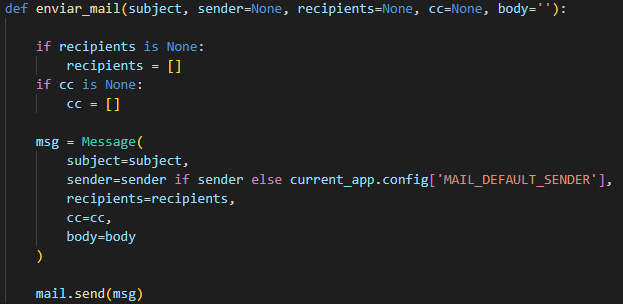
\includegraphics[width=0.5\textwidth]{img/desarrollo/mailpy.png}
            \caption{Código de la función de envío de correos electrónicos.}
            \label{fig:5.9}
        \end{figure}

    \subsection{Implementación e integración del bot de Discord}
        